\documentclass[a4paper,11pt]{article}

% Packages essentiels
\usepackage[utf8]{inputenc}
\usepackage[T1]{fontenc}
\usepackage[numbers]{natbib}
\usepackage[french]{babel}
\usepackage{csquotes}
\usepackage{xcolor}
\usepackage{graphicx}
\usepackage{tabularx}
\usepackage{makecell}
\usepackage{booktabs}
\usepackage{array}
\usepackage{amsmath,amssymb,amsfonts}
\usepackage{float}
\usepackage{listings}
\usepackage{tcolorbox}
\usepackage{pgfplots}
\usepackage{parskip}
\usepackage[french]{datetime2}
\usepackage{multirow}
\usepackage{siunitx}
\usepackage{mdframed}
\usepackage{tocloft}  % Ajout du package pour la table des matières
\usepackage[colorlinks=true,breaklinks=true]{hyperref}
\usepackage[nameinlink]{cleveref}
\usepackage{fontawesome5}
\usepackage{adjustbox}

% Configuration de la table des matières
\renewcommand{\cftsecleader}{\cftdotfill{\cftdotsep}}
\renewcommand{\cftsecpagefont}{\normalfont}
\renewcommand{\cftsecfont}{\normalfont}

% Configuration de pgfplots
\pgfplotsset{compat=newest,compat/show suggested version=false}

% Configuration des boîtes de texte
\newmdenv[
    linewidth=1pt,
    topline=true,
    bottomline=true,
    leftline=true,
    rightline=true,
    backgroundcolor=gray!5,
    innertopmargin=10pt,
    innerbottommargin=10pt,
    innerrightmargin=10pt,
    innerleftmargin=10pt,
    skipabove=15pt,
    skipbelow=15pt
]{solution}

% Configuration améliorée pour listings
\lstdefinestyle{mystyle}{
    basicstyle=\ttfamily\footnotesize,
    backgroundcolor=\color{gray!10},
    frame=single,
    framesep=3pt,
    breaklines=true,
    showstringspaces=false,
    keywordstyle=\color{blue},
    stringstyle=\color{red},
    commentstyle=\color{green!60!black},
    captionpos=b,
    literate={é}{{\'e}}1 {è}{{\`e}}1 {à}{{\`a}}1 {É}{{\'E}}1 {ù}{{\'u}}1
    {ê}{{\^e}}1
    {Ê}{{\^E}}1
    {π}{{$\pi$}}1
    {≤}{{$\leq$}}1
    {≥}{{$\geq$}}1
    {≠}{{$\neq$}}1
    {²}{{$^2$}}1
    {⁸}{{$^8$}}1
    {⁷}{{$^7$}}1
    {⁶}{{$^6$}}1
    {⁵}{{$^5$}}1
    {⁴}{{$^4$}}1
    {³}{{$^3$}}1
}
\lstset{style=mystyle}

% Configuration des marges
\usepackage[top=2cm, bottom=2cm, left=2.5cm, right=2.5cm]{geometry}

% Définition des environnements personnalisés
\newtcolorbox{graysection}[1]{
    colback=gray!10,
    colframe=white,
    title=#1,
    fonttitle=\bfseries\large,
    boxrule=0pt,
    arc=0pt,
    boxsep=5pt,
    left=10pt,right=10pt,top=10pt,bottom=10pt
}

% Commande TODO professionnelle
\newcommand{\todo}[1]{\textcolor{red}{\bfseries [TODO: #1]}}

% Informations du document
\newcommand{\titre}{
Agent conversationnel pour l'interrogation de la base de données Open Food Facts \\
\vspace{1cm} Rapport final}
\newcommand{\auteurs}{Alain Boisvert}
\newcommand{\matricules}{994 029 313}
\newcommand{\destinataire}{Luc Lamontagne}
\newcommand{\cours}{IFT-6005 - Projet intégrateur}
\newcommand{\dateremise}{7 avril 2025}

\title{IFT-6005 - Projet intégrateur - H25 \\ ~ \\ Agent conversationnel pour l'interrogation de la base de données Open Food Facts}
\author{Alain Boisvert}
\date{2 mars 2025}

\begin{document}

\thispagestyle{empty}  % Pour éviter d'avoir un en-tête et un pied de page sur la page couverture

\includegraphics[width=5cm]{./figures/logo.jpg}	 % Pour inclure le logo de l'Université Laval
\vspace{4cm}  % Espacement vertical
\begin{center}	% On centre le texte
    \setlength{\baselineskip}{2.0\baselineskip}  % Multiplie l'interligne par 1.5
{\LARGE \bf \titre} \\  % \huge fait que le texte est gros, \bf fait que le texte est gras
\vspace{4cm}
\large Travail présenté à \destinataire \\ \vspace{0.3cm} \cours\\
\vspace{4cm}
% réalisé par \\ \auteurs ;\\ \matricules
{\large réalisé par \\ \vspace{0.3cm} \auteurs \\  \vspace{0.3cm} \matricules}
\vfill	% On va jusqu'au bas de la page avant de mettre le texte ci-dessous
{\large \dateremise} 
\pagebreak
\end{center}

\newpage
% \maketitle

% Table des matières
\tableofcontents
\newpage

%----------------------------------------------------------------------------------------
\section{Introduction}  
\label{sec:probleme}

L'accès aux informations nutritionnelles reste souvent limité par des interfaces techniques
nécessitant des compétences en langages de requête comme SQL. Cette barrière empêche de nombreux
utilisateurs d'exploiter pleinement des bases de données 
comme Open Food Facts\footnote{\url{https://world.openfoodfacts.org/}}, 
qui contient des informations détaillées sur des milliers de produits alimentaires. 

Ce projet vise à développer un agent conversationnel utilisant des grands modèles de langage (LLM) 
pour permettre aux utilisateurs de poser des questions en langage naturel 
comme (\textit{\enquote{Quelles collations sans allergènes ont un Nutri-score A ?}}). 
Cette approche démocratise l'accès aux données nutritionnelles tout en améliorant la qualité
des réponses grâce à l'exploitation directe de sources structurées. 

Ce rapport de mi-session présente l'état d'avancement du projet à la mi-session, les défis rencontrés et les solutions implémentées.


%----------------------------------------------------------------------------------------
\part{Interrogation de la base avec DuckDB}
\label{part:duckdb}

Cette première partie du rapport, réalisée lors de la première moitié du semestre, présente l'approche d'interrogation de la base de données Open Food Facts à l'aide de DuckDB et d'un agent conversationnel basé sur un LLM.


%----------------------------------------------------------------------------------------
\section{Rappel de l'objectif du projet}
\label{sec:revue}

L'objectif de ce projet est de développer un agent conversationnel permettant aux utilisateurs 
d'interroger la base de données Open Food Facts en langage naturel. Le système doit comprendre les 
questions des utilisateurs sur les produits alimentaires, les convertir en requêtes SQL, et fournir
des réponses claires et précises. Les données manquantes ou incomplètes doivent être compensées 
par une recherche alternative 
dans le Guide alimentaire canadien\footnote{\url{https://guide-alimentaire.canada.ca/fr/}}.




% ----------------------------------------------------------------------------------------
\section{Approche proposée}
\label{sec:approche}

\subsection{Architecture du système}

L'architecture modulaire du système comprend les composants suivants :

\begin{itemize}
    \item \textbf{Module de dialogue :} Gère les conversations avec l'utilisateur en utilisant un LLM pré-entraîné.
    \item \textbf{Convertisseur texte-SQL :} Transforme les questions en requêtes SQL adaptées à 
    Open Food Facts. Il utilise d'abord une recherche sémantique dans un dictionnaire de données pour trouver les colonnes pertinentes.
    \item \textbf{Connecteur de base de données :} Communique avec DuckDB pour exécuter les requêtes. Les requêtes SQL sont vérifiées avant exécution pour garantir leur sécurité.
    \item \textbf{Recherche sur le Web :} Consulte le Guide alimentaire canadien quand les informations manquent dans la base de données.
    \item \textbf{Générateur de réponses :} Transforme les résultats bruts en réponses naturelles, en précisant les sources.
\end{itemize}

La figure \ref{fig:architecture} présente l'architecture modulaire du système, illustrant comment les questions des utilisateurs sont traitées par le module de dialogue LLM, enrichies par la recherche sémantique des colonnes pertinentes, puis converties en requêtes SQL pour interroger Open Food Facts, avec un repli vers le Guide alimentaire canadien lorsque nécessaire.

\begin{figure}[H]
    \centering
    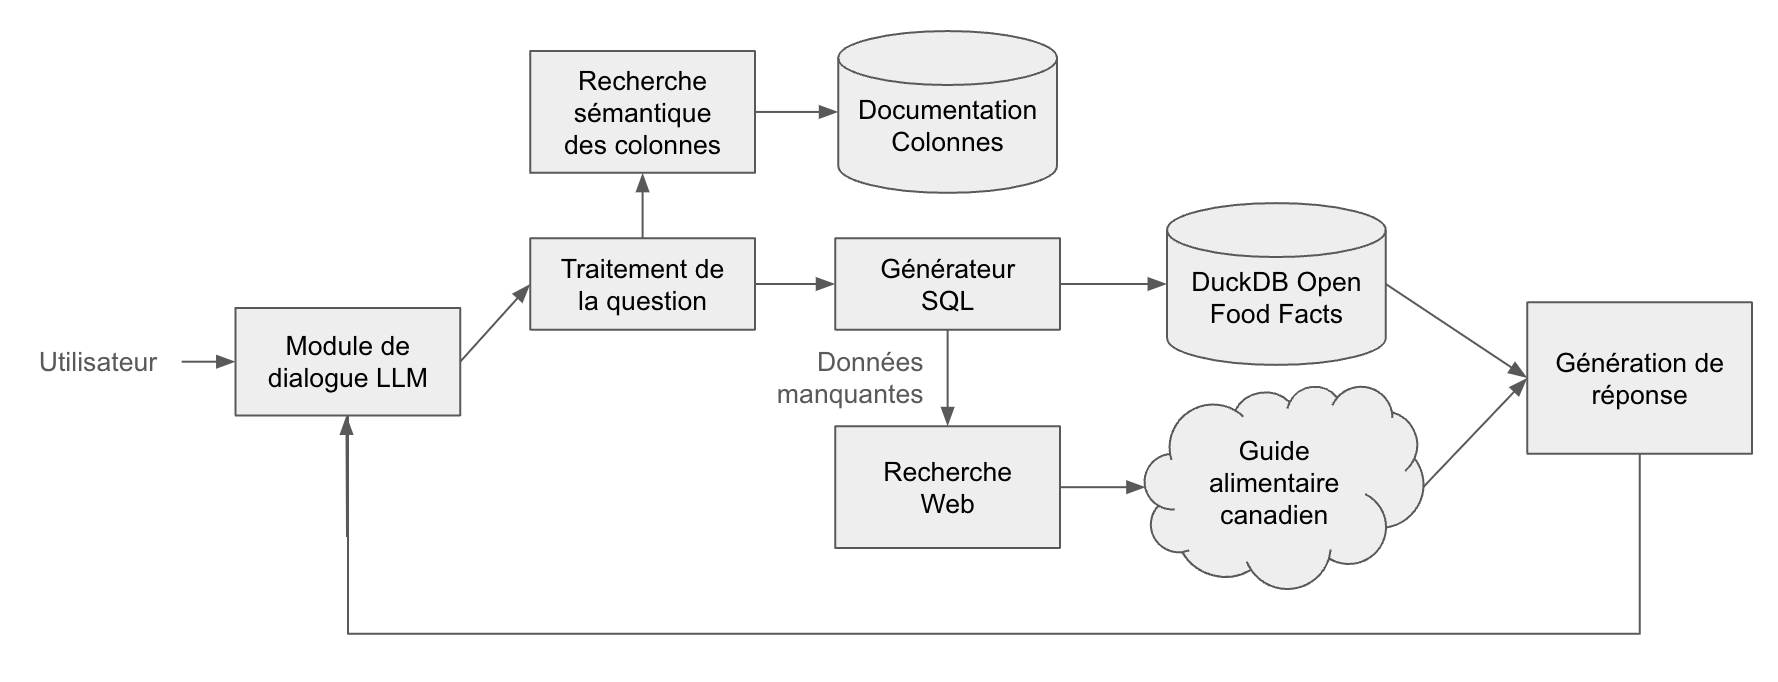
\includegraphics[width=0.95\textwidth]{figures/architecture-agent.png}
    \caption{Architecture du système d'agent conversationnel pour l'interrogation d'Open Food Facts}
    \label{fig:architecture}
\end{figure}

\subsection{Sélection des technologies}

J'ai choisi ces technologies pour mon projet :

\begin{itemize}
    \item \textbf{DuckDB} comme base de données, car :
    \begin{itemize}
        \item Elle est rapide pour les requêtes analytiques
        \item Elle gère bien la mémoire
        \item Elle supporte les fichiers Parquet et les requêtes SQL complexes
    \end{itemize}
    \item \textbf{Hugging Face Smolagents} comme framework d'agent, car :
    \begin{itemize}
        \item Il est simple à utiliser
        \item Il permet d'intégrer différents LLMs et outils
        \item Il est bien documenté et supporté
    \end{itemize}
    \item \textbf{Modèles de langage} :
    \begin{itemize}
        \item Pour le développement : \detokenize{Llama3.1:8B-Instruct} via Ollama (en local)
        \item Pour les tests : \detokenize{Llama3.1:8B-Instruct} et \detokenize{Qwen2.5:7B} via Ollama (en local), et Claude 3.5 Sonnet (modèle commercial via API)
        \item Cette approche limite les coûts d'API
    \end{itemize}
    \item \textbf{FAISS} pour la recherche sémantique :
    \begin{itemize}
        \item Il identifie rapidement les colonnes pertinentes pour chaque question
        \item Il transforme la documentation des colonnes en vecteurs faciles à comparer
    \end{itemize}
\end{itemize}

Notons qu'au début du projet, j'envisageais d'utiliser CrewAI\footnote{\url{https://www.crewai.com/open-source}} pour l'orchestration des agents, mais j'ai finalement opté pour SmolAgents pour sa simplicité et sa flexibilité.
Contrairement à CrewAI, qui impose une structure rigide avec des rôles prédéfinis, SmolAgents permet une approche plus modulaire où les agents interagissent librement via des outils définis par l’utilisateur. 
De plus, il s’intègre facilement aux outils déjà utilisés dans le projet et évite la complexité d’une organisation centralisée, ce qui rend le développement plus rapide et plus facile.

Aucune alternative à FAISS n’a été envisagée, car cette bibliothèque répond parfaitement aux besoins du projet. Elle est open-source, largement reconnue, soutenue par Facebook et simple à utiliser, tout en offrant d’excellentes performances pour la recherche sémantique.


% ----------------------------------------------------------------------------------------
\newpage
\section{État d'avancement et tâches réalisées}
\label{sec:progress}

Le développement de l'agent conversationnel a progressé significativement durant cette
première phase du projet. Cette section détaille les différentes tâches accomplies
et leur état d'avancement, en suivant le plan initial.

% Section 4.1
\subsection{Mise en place de l'environnement de développement}

J'ai d'abord créé un environnement de développement complet :

\begin{itemize}
    \item \textbf{Infrastructure et outils}
    \begin{itemize}
        \item Un dépôt GitHub\footnote{\url{https://github.com/boisalai/ift-6005}} pour le code et la documentation
        \item Un environnement virtuel Python avec les bonnes dépendances
        \item Des outils comme Black pour le formatage et Pylint pour l'analyse de code
    \end{itemize}
    \item \textbf{Dépendances principales}
    \begin{itemize}
        \item DuckDB pour la base de données
        \item Smolagents\footnote{\url{https://github.com/huggingface/smolagents}} pour le framework d'agent
        \item FAISS\footnote{\url{https://github.com/facebookresearch/faiss}} pour la recherche sémantique
        \item Les bibliothèques habituelles pour l'analyse de données et le traitement du langage
    \end{itemize}
    \item \textbf{Configuration des API}
    \begin{itemize}
        \item Des variables d'environnement pour les clés API dans un fichier \texttt{.env}
        \item L'accès à l'API d'Anthropic pour Claude 3.5 Sonnet
        \item L'interface avec Ollama pour les tests locaux
    \end{itemize}
\end{itemize}


% Section 4.2
\subsection{Préparation de la base de données}

J'ai téléchargé le fichier Parquet d'Open Food Facts (3,6~millions de produits) :

\begin{lstlisting}[language=bash, caption=Téléchargement du fichier Parquet]
wget -P data/ https://huggingface.co/datasets/openfoodfacts/product-database/resolve/main/food.parquet
\end{lstlisting}

Ensuite, j'ai converti le fichier Parquet en base DuckDB pour faciliter les requêtes SQL :

\begin{lstlisting}[language=Python, caption=Conversion en base DuckDB]
DATA_DIR = Path("../data")
PARQUET_PATH = DATA_DIR / "food.parquet"
FULL_DB_PATH = DATA_DIR / "food_full.duckdb"

con = duckdb.connect(str(FULL_DB_PATH), config={'memory_limit': '8GB'})
con.execute(f"CREATE TABLE products AS SELECT * FROM '{PARQUET_PATH}'")
con.close()
\end{lstlisting}

Pour accélérer les requêtes, j'ai créé une version avec seulement les 94\,802~produits canadiens :

\begin{lstlisting}[language=Python]
FILTERED_DB_PATH = DATA_DIR / "food_canada.duckdb"

con = duckdb.connect(str(FILTERED_DB_PATH))
con.execute(f"ATTACH DATABASE '{FULL_DB_PATH}' AS full_db")
con.execute(f"""
    CREATE TABLE products AS 
    SELECT * FROM full_db.products
    WHERE array_contains(countries_tags, 'en:canada')
""")
\end{lstlisting}

La création des bases DuckDB s'effectue via le script \texttt{data.py}.

J'ai aussi analysé les données et découvert que certaines colonnes sont très complètes (>~95\%) alors que d'autres sont peu renseignées (<~30\%).

\begin{figure}[htbp]
    \centering
    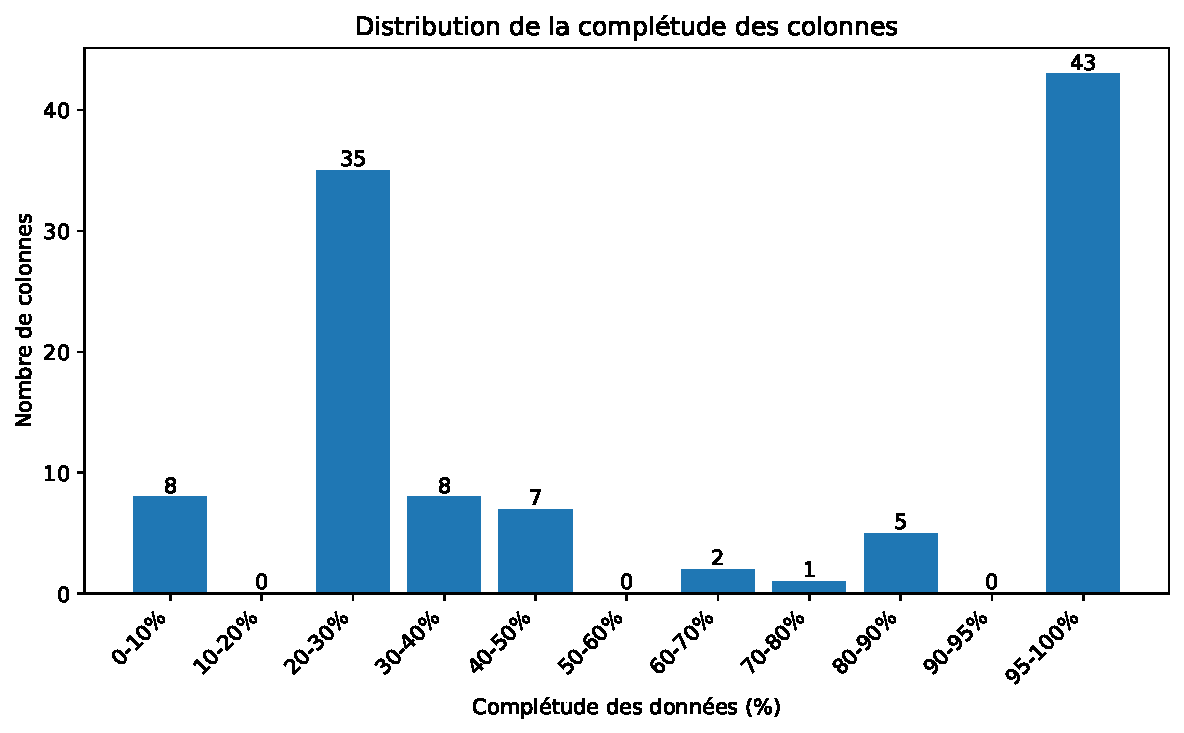
\includegraphics[width=0.9\textwidth]{figures/missing_values.pdf}
    \caption{Distribution de la complétude des colonnes de la base de données}
    \label{fig:missing-values}
\end{figure}

J'ai également remarqué que certaines colonnes ont des structures complexes. 
Par exemple, la colonne \texttt{categories} contient du texte libre séparé par des virgules, alors que \texttt{categories\_tags} contient des identifiants standardisés incluant des préfixes de langue.

Exemple de données pour la colonne \texttt{categories} :

\begin{lstlisting}
"Sweeteners,Syrups,Simple syrups,Agave syrups"
"Plant-based beverages,Fruit-based,Juices and nectars,Fruit juices,Lemon juice"
"Snacks,Sweet snacks,Biscuits and cakes,Cakes"
\end{lstlisting}

Exemple de données pour la colonne \texttt{categories\_tags} :

\begin{lstlisting}
["en:plant-based-foods-and-beverages", "en:beverages", 
    "en:plant-based-beverages", "en:coconut-milks"]
["en:snacks", "en:sweet-snacks", "en:cocoa-and-chocolate-products", 
    "en:chocolates"]
["en:dairies", "en:milk", "en:whole-milk"]
\end{lstlisting}



% Section 4.3

\subsection{Documentation des données}

J'ai créé un dictionnaire détaillé
(\texttt{columns\_documentation.json}) pour aider l'agent à générer des requêtes SQL. Il contient des informations sur chacune des 109~colonnes.
La documentation pour chaque colonne ressemble à ceci :

\newpage
\begin{lstlisting}
"nova_groups_tags": {
  "type": "VARCHAR[]",
  "description": "Array containing NOVA food classification group tags. NOVA...",
  "examples": [
    "['en:1-unprocessed-or-minimally-processed-foods']",
    "['en:4-ultra-processed-food-and-drink-products']",
    "['en:3-processed-foods']"
  ],
  "is_nullable": true,
  "common_queries": [
    {
      "description": "Distribution of products across NOVA groups",
      "sql": "SELECT nova_groups_tags, COUNT(*) as product_count FROM products..."
    },
    /* Autres... */
  ]
},
\end{lstlisting}

Cette documentation est générée par un agent qui :

\begin{itemize}
    \item Interroge la colonne dans la base de données
    \item Recherche des informations sur le site Open Food Facts
    \item Propose une description de la colonne
    \item Génère des requêtes SQL typiques
    \item Ajoute la documentation au fichier JSON
\end{itemize}

Ces tâches s'effectuent via le script \texttt{docoff.py}.


% Section 4.4
\subsection{Création du jeu de test}

J'ai créé un jeu de 100~questions-réponses en anglais et en français 
en utilisant les requêtes SQL documentées à l'étape précédente. 
Pour chaque requête SQL, un agent:

\begin{itemize}
    \item Évalue si la requête répond à une question pertinente pour un consommateur
    \item Génère des questions en français et en anglais
    \item Crée des réponses claires correspondant à la requête SQL
    \item Vérifie que les résultats de la requête permettent de répondre à la question
\end{itemize}

\newpage
Les paires sont stockées dans \texttt{qa\_pairs.json} avec cette structure:

\begin{lstlisting}
{
  "column": "nutriscore_score",
  "sql": "SELECT code, product_name, nutriscore_score FROM products WHERE nutriscore_score IS NOT NULL ORDER BY nutriscore_score ASC LIMIT 50",
  "questions": {
    "fr": "Quels sont les produits alimentaires les plus sains selon le Nutri-Score ?",
    "en": "What are the healthiest food products according to the Nutri-Score?"
  },
  "answers": {
    "fr": "D'après les résultats, les produits les plus sains sont principalement des légumineuses comme les lentilles rouges et les pois jaunes cassés, avec un Nutri-Score de -17, ce qui est excellent.",
    "en": "According to the results, the healthiest products are mainly legumes such as red split lentils and yellow split peas, with a Nutri-Score of -17, which is excellent."
  }
},
/* Autres... */
\end{lstlisting}

Le jeu de 100~questions-réponses est créé avec le script \texttt{question\_answer.py}.


% Section 4.5
\subsection{Développement de la recherche sémantique}

J'ai implémenté une recherche sémantique avec FAISS et le modèle \texttt{all-MiniLM-L6-v2} pour identifier les colonnes pertinentes dans la base de données :

\begin{itemize}
    \item \textbf{Préparation des embeddings}
    \begin{itemize}
        \item La documentation des 109 colonnes est convertie en vecteurs
        \item Le modèle MiniLM génère des embeddings de dimension 384
        \item Ce modèle multilingue fonctionne en français et en anglais
    \end{itemize}
    
    \item \textbf{Indexation FAISS}
    \begin{itemize}
        \item Un index est créé pour les recherches rapides par similarité
        \item Les embeddings sont sauvegardés dans des fichiers pour éviter de recalculer l'index
    \end{itemize}
    
    \item \textbf{Processus de recherche}
    \begin{itemize}
        \item Pour chaque question, l'embedding de la question est comparé à ceux des colonnes
        \item Les 5 colonnes les plus similaires sont retournées avec un score
        \item Seules les colonnes avec un score > 0.5 sont utilisées
    \end{itemize}
\end{itemize}

Les résultats de cette recherche sont ajoutés au prompt de l'agent pour l'aider à générer de meilleures requêtes SQL.

Cette approche s'inspire des travaux de \citet{gao2023text} sur l'apprentissage contextuel (\textit{in-context learning}) pour Text-to-SQL, en adoptant une méthode similaire où l'agent identifie d'abord les colonnes sémantiquement pertinentes pour la question posée, puis utilise ces informations avec des exemples de requêtes SQL dans le prompt afin d'améliorer la qualité de la conversion du langage naturel vers SQL.


% Section 4.6
\subsection{Création des outils d'agent}

Un agent intelligent est un logiciel qui peut interagir avec son environnement, collecter des données et les utiliser pour effectuer des tâches autodéterminées afin d'atteindre des objectifs prédéterminés.

J'ai choisi Smolagents pour son approche simple et flexible. Cet outil est idéal pour expérimenter rapidement avec la logique d'agent, particulièrement lorsque l'application est relativement simple.

\newpage
J'ai développé deux outils pour l'agent :

\begin{itemize}
    \item \textbf{Exécution SQL sécurisée} : Permet à l'agent de générer et d'exécuter des requêtes SQL sur DuckDB avec des vérifications de sécurité
    \item \textbf{Recherche sur le Web} : Permet à l'agent de consulter le Guide alimentaire canadien quand les informations ne sont pas dans Open Food Facts
\end{itemize}


% Section 4.7
\subsection{Stratégie d'évaluation}

J'évalue l'agent selon quatre métriques principales :

\begin{itemize}
    \item \textbf{Précision d'exécution (EX)} : Mesure si l'agent génère des requêtes SQL correctes 
    avec la pondération suivante :
    \begin{itemize}
        \item 20\% pour avoir une requête
        \item 30\% pour l'exécution sans erreur
        \item 50\% pour des résultats corrects
    \end{itemize}
    
    \item \textbf{Précision sémantique (PS)} : Compare la similarité entre les réponses de l'agent et les réponses attendues
    
    \item \textbf{Respect de séquence (RS)} : Vérifie si l'agent suit une stratégie de recherche cohérente (d'abord la base de données, puis le Guide alimentaire canadien)
    
    \item \textbf{Temps de réponse moyen (TRM)} : Mesure la rapidité du traitement
\end{itemize}


% Section 4.8
\subsection{Avancement par rapport à la planification initiale}

Voici un tableau comparatif entre la planification initiale et l'état actuel du projet :

\begin{itemize}
    \item \textbf{Mise en place de l'environnement}
    \begin{itemize}
        \item \textbf{Planification initiale} : 5h -- Environnement Python, GitHub\footnote{\url{https://github.com/boisalai/ift-6005}}
        \item \textbf{État actuel} : Environnement configuré, GitHub prêt, Black \& Pylint utilisés
        \item \textbf{Statut} : Terminé $\checkmark$
    \end{itemize}
    
    \item \textbf{Préparation de la base de données}
    \begin{itemize}
        \item \textbf{Planification initiale} : 5h -- Création d'une base DuckDB
        \item \textbf{État actuel} : Base DuckDB créée avec filtrage des produits canadiens. Voir le script \texttt{data.py}
        \item \textbf{Statut} : Terminé $\checkmark$
      \end{itemize}
    
    \item \textbf{Création du jeu de test (100 questions)}
    \begin{itemize}
        \item \textbf{Planification initiale} : 10h -- Générer des questions et requêtes SQL
        \item \textbf{État actuel} : 100 questions-réponses créées en français et anglais. Voir le script \texttt{question\_answer.json} et le fichier \texttt{qa\_pairs.json}
        \item \textbf{Statut} : Terminé $\checkmark$
    \end{itemize}
    
    \item \textbf{Documentation des données}
    \begin{itemize}
        \item \textbf{Planification initiale} : Prévoir un dictionnaire des colonnes
        \item \textbf{État actuel} : Documentation détaillée (109 colonnes, exemples, SQL). Voir le script \texttt{docoff.py} et le fichier \texttt{columns\_documentation.json}
        \item \textbf{Statut} : Terminé $\checkmark$
    \end{itemize}
    
    \item \textbf{Développement de la conversion texte-SQL}
    \begin{itemize}
        \item \textbf{Planification initiale} : 25h -- Approche texte-SQL avec LLM
        \item \textbf{État actuel} : Implémentation avec FAISS pour recherche sémantique. Voir le script \texttt{evaluation\_04.py}
        \item \textbf{Statut} : Terminé $\checkmark$
    \end{itemize}
    
    \item \textbf{Développement du module de dialogue}
    \begin{itemize}
        \item \textbf{Planification initiale} : 20h -- Utilisation de Qwen2-7B-Instruct
        \item \textbf{État actuel} : Utilisation de \detokenize{Llama3.1:8B}, \detokenize{Qwen2.5:7B}, Claude 3.5. Voir le script \texttt{evaluation\_04.py}
        \item \textbf{Statut} : Terminé $\checkmark$
    \end{itemize}
    
    \item \textbf{Implémentation du générateur de réponses}
    \begin{itemize}
        \item \textbf{Planification initiale} : 25h -- Transformer résultats SQL en texte
        \item \textbf{État actuel} : Fonctionnel avec SmolAgents et intégration Guide alimentaire canadien. Voir le script \texttt{evaluation\_04.py}
        \item \textbf{Statut} : Terminé $\checkmark$
    \end{itemize}
    
    \item \textbf{Stratégie d'évaluation (métriques EX, PS, RS, TRM)}
    \begin{itemize}
        \item \textbf{Planification initiale} : 10h -- Définir et tester les métriques
        \item \textbf{État actuel} : Métriques définies et tests réalisés sur plusieurs modèles. Voir le script \texttt{evaluation\_04.py}
        \item \textbf{Statut} : Terminé $\checkmark$
    \end{itemize}
    
    \item \textbf{Optimisation des requêtes SQL et prompts}
    \begin{itemize}
        \item \textbf{Planification initiale} : 15h -- Améliorer la génération SQL
        \item \textbf{État actuel} : Ajustements des prompts et meilleure gestion des colonnes SQL. Voir le script \texttt{evaluation\_04.py}
        \item \textbf{Statut} : Terminé $\checkmark$
    \end{itemize}
    
    \item \textbf{Gestion des données manquantes}
    \begin{itemize}
        \item \textbf{Planification initiale} : 15h -- Trouver des stratégies alternatives
        \item \textbf{État actuel} : Approche hybride avec Guide alimentaire canadien intégrée. Voir le script \texttt{evaluation\_04.py}
        \item \textbf{Statut} : Terminé $\checkmark$
    \end{itemize}
    
    \item \textbf{Sélection dynamique de LLM}
    \begin{itemize}
        \item \textbf{Planification initiale} : 10h -- Tester plusieurs modèles pour équilibre coût/performance
        \item \textbf{État actuel} : Non réalisé.
        \item \textbf{Statut} : Non réalisé.
    \end{itemize}
    
    \item \textbf{Exploration de nouvelles méthodes (ex. RAG, Neo4j)}
    \begin{itemize}
        \item \textbf{Planification initiale} : Optionnelle en phase avancée
        \item \textbf{État actuel} : Mentionnée comme piste future
        \item \textbf{Statut} : À explorer
    \end{itemize}
\end{itemize}

En résumé, les tâches principales sont terminées selon la planification. Les optimisations avancées et l’exploration de nouvelles approches (ex. RAG) sont encore à explorer. 


%----------------------------------------------------------------------------------------
% Section 5
\section{Résultats et discussion}
\label{sec:results}

Le tableau suivant résume les résultats des tests effectués sur l'agent conversationnel en utilisant différents modèles de langage et en évaluant les métriques EX, PS, RS et TRM
sur 20~questions pour chaque modèle, en français et en anglais.

J'ai limité les tests à 20 questions par modèle afin de réduire les coûts d'API associés aumodèle commercial Claude 3.5 Sonnet. Tous les tests ont été réalisés sur un MacBook Pro M1 équipé de 16~Go de RAM.


\begin{table}[h!]
\small
\centering
\begin{tabular}{l|r r|r r|r r}
\toprule
& \multicolumn{2}{c|}{\detokenize{Llama3.1:8B}} & \multicolumn{2}{c|}{\detokenize{Qwen2.5:7B}} 
& \multicolumn{2}{c}{\makecell{Claude 3.5 \\ Sonnet}} \\
& {en} & {fr} & {en} & {fr} & {en} & {fr} \\
\midrule
Nombre de questions & 20 & 20 & 20 & 20 & 20 & 20 \\
Précision d'exécution (EX) (\%) & 31.1 & 25.0 & 28.6 & 40.0 & 42.5 & 47.5 \\
Précision sémantique (PS) (\%) & 16.7 & 20.0 & 66.5 & 49.5 & 62.3 & 54.7 \\
Respect de séquence (RS) (\%) & 100.0 & 100.0 & 100.0 & 100.0 & 100.0 & 100.0 \\
Temps de réponse moyen (TRM) & 432~s & 273~s & 239~s & 201~s & 37~s & 41~s \\
\bottomrule
\end{tabular}
\caption{Résultats des tests sur différents modèles de langage}
\label{tab:resultats}
\end{table}

\newpage
Ici \detokenize{Llama3.1:8B} réfère au modèle \texttt{ollama/llama3.1:8B-instruct-q8\_0}, 
\detokenize{Qwen2.5:7B} au modèle \texttt{ollama/qwen2.5:7B-instruct} et 
\detokenize{Claude 3.5 Sonnet} au modèle \\
\texttt{anthropic/claude-3-5-sonnet-20241022}.



Les principales observations sont les suivantes :

\begin{itemize}
\item \textbf{Performance des modèles} : Claude 3.5 Sonnet surpasse significativement les modèles \detokenize{Llama3.1:8B} et \detokenize{Qwen2.5:7B} sur presque toutes les métriques, particulièrement en précision d'exécution (EX) et en temps de réponse moyen (TRM).
\item \textbf{Différences linguistiques} : Les performances varient selon la langue. Les résultats en français montrent généralement une bonne précision d'exécution pour Claude 3.5 Sonnet et \detokenize{Qwen2.5:7B} par rapport à l'anglais, suggérant une bonne capacité de traitement multilingue.
\item \textbf{Respect de séquence} : Tous les modèles obtiennent un score parfait (100~\%) sur le respect de séquence (RS), indiquant que la stratégie de recherche définie est bien suivie indépendamment du modèle utilisé.
\item \textbf{Précision sémantique} : \detokenize{Qwen2.5:7B} surpasse remarquablement \detokenize{Llama3.1:8B} en précision sémantique, particulièrement en anglais (66,5\,\% contre 16,7\,\%), suggérant peut-être une meilleure compréhension du domaine des produits alimentaires.
\end{itemize}

Ces résultats démontrent clairement l'avantage d'utiliser un modèle commercial comme Claude 3.5 Sonnet pour des applications pratiques, bien que \detokenize{Qwen2.5:7B} offre une alternative gratuite intéressante avec des performances acceptables, particulièrement pour la compréhension sémantique.
Ces évaluations s'effectuent dans le script \texttt{evaluation\_04.py}.


%----------------------------------------------------------------------------------------
% Section 6
\section{Problèmes rencontrés et solutions}
\label{sec:problems}

\subsection{Complexité structurelle des données}

Un défi majeur a été de comprendre les structures complexes d'Open Food Facts. Sans documentation officielle complète, j'ai dû explorer la base en détail pour décoder des colonnes et 
comprendre les relations entre les colonnes.
La base contient des structures hétérogènes, comme les colonnes \texttt{categories} et \texttt{categories\_tags}. Cette complexité rend difficile la génération de bonnes requêtes SQL.

Pour résoudre ce problème, j'ai créé une documentation détaillée de la base de données 
avec pour chaque colonne :
\begin{itemize}
\item Le type de données et sa description
\item Des exemples de valeurs
\item Des modèles de requêtes SQL adaptées
\end{itemize}

Comme mentionné précédemment, les colonnes pertinentes pour une question de l'utilisateur sont identifiées par une recherche sémantique, puis utilisées pour enrichir le prompt de l'agent. 

\vskip 0.1cm
Je pense qu'on peut encore améliorer cette documentation, peut-être avec plus d'exemples annotés.

\subsection{Limitations des modèles de langage légers}

L'utilisation d'un modèle léger et gratuit (\detokenize{Llama3.1:8B}) pendant le développement a permis d'avancer sans coûts d'API, mais a montré des limites :
\begin{itemize}
\item Difficulté à comprendre des instructions complexes
\item Problèmes pour maintenir un format de réponse cohérent
\item Génération SQL parfois incorrecte
\item Difficulté à suivre des séquences d'actions
\end{itemize}

\vskip 0.1cm
Pour résoudre ces problèmes, j'ai :
\begin{itemize}
\item Amélioré les prompts: Instructions plus simples et directes, avec plus d'exemples
\item Modifié l'architecture: Utilisé les mécanismes de MultiStepAgent de Smolagents pour mieux suivre la progression
\end{itemize}

\vskip 0.1cm
Des tests avec Claude 3.5 Sonnet montrent des résultats bien meilleurs, confirmant l'intérêt d'une approche hybride : développement avec des modèles légers, puis déploiement avec des modèles plus puissants.



%----------------------------------------------------------------------------------------
% Section 7
\section{Prochaines étapes}
\label{sec:next}

Si je continue ce projet sur cette voie, je peux :
\begin{itemize}
\item \textbf{Mieux documenter la structure de la base de données} : Créer une meilleure carte des relations entre colonnes, ajouter des exemples pour les structures difficiles, et enrichir la documentation avec des informations sur la distribution des données.
\item \textbf{Optimiser la recherche sémantique} : Ajouter une recherche vectorielle sur les fiches produits en plus de l'approche SQL. Cela aiderait à trouver des produits similaires quand les requêtes SQL sont limitées.
\end{itemize}

\vskip 0.1cm
Je pourrais aussi explorer une approche différente avec \textbf{RAG sur un graphe de connaissances} en utilisant Neo4j\footnote{\url{https://neo4j.com/}} et 
Langchain\footnote{\url{https://www.langchain.com/}}. Cette méthode pourrait mieux représenter les relations complexes entre produits et informations nutritionnelles.






%----------------------------------------------------------------------------------------
\part{Graphe de produits alimentaires avec recherche sémantique}
\label{part:graphe}

Pour la seconde partie du projet, j'ai exploré l'utilisation d'un graphe avec recherche sémantique comme alternative à l'approche DuckDB présentée précédemment. Cette section décrit la mise en œuvre et l'évaluation de cette approche.

\section{Avantages potentiels d'un graphe de connaissances}
\label{sec:avantages-graphe}

Un graphe de connaissances présenterait potentiellement plusieurs avantages par rapport à une base de données relationnelle ou DuckDB pour notre cas d'usage :

\begin{itemize}
    \item \textbf{Représentation des relations} : Les données alimentaires étant intrinsèquement relationnelles, un graphe pourrait modéliser plus naturellement les liens entre produits, ingrédients et catégories.
    
    \item \textbf{Requêtes complexes} : Les requêtes à plusieurs niveaux de relations seraient potentiellement plus intuitives à exprimer comme parcours de graphe qu'avec des jointures SQL.
    
    \item \textbf{Flexibilité et évolutivité} : L'ajout de nouvelles relations ou propriétés serait simplifié, sans nécessiter de restructuration complète du schéma.
\end{itemize}



\newpage

\section{Lien avec les recherches récentes}
\label{sec:recherches}

L'article \citet{mohammadjafari2024natural} sur l'utilisation des LLMs pour la génération de SQL confirme l'intérêt des graphes de connaissances. Dans la section IV intitulée « LEVERAGING KNOWLEDGE GRAPHS IN LLM-BASED TEXT-TO-SQL SYSTEM », les auteurs décrivent plusieurs avantages :

\begin{itemize}
    \item \textbf{Représentation structurée des entités et relations} : « Knowledge Graphs are structured representations of real-world entities and relationships between them, serving as a rich repository that connects and organizes semantic concepts. They provide, in a database context, a way of navigating through complex relationships and hierarchical structures that can represent large volumes of structured data effectively » \citep{mohammadjafari2024natural}.
    
    \item \textbf{Liaison de schéma améliorée} : « Knowledge graphs allow large language models to link natural language queries with the respective tables and columns of the database schema through explicit semantic relations from diverse entities » \citep{mohammadjafari2024natural}.
    
    \item \textbf{Enrichissement contextuel} : « Knowledge graphs provide that additional layer of context necessary for an LLM to disambiguate terms in NL queries. This context permits the model to resolve references to entities or relationships that may not be immediately obvious from the query itself and hence improve the accuracy of the generated SQL » \citep{mohammadjafari2024natural}.
\end{itemize}

Ces avantages sont pertinents pour notre projet, où la compréhension du 
contexte des produits alimentaires (relations entre produits, ingrédients, catégories, etc.) est essentielle pour répondre correctement aux questions des utilisateurs.


\section{Choix de la technologie de graphe}
\label{sec:choix-graphe}

J'ai d'abord envisagé Neo4j\footnote{\url{https://neo4j.com/}}, base de données orientée graphe populaire, pour créer un graphe de produits alimentaires. Cependant, après plusieurs essais, j'ai rencontré des limitations avec la version gratuite de Neo4j qui restreint le nombre de relations pouvant être créées. Ces contraintes m'obligeaient à réduire significativement le nombre de produits canadiens, rendant impossible une comparaison équitable avec l'approche DuckDB.

Malgré une tentative avec une version payante de Neo4j, le temps de création du graphe s'est avéré excessivement long, probablement en raison de la localisation du serveur distant.

Pour contourner ces obstacles, j'ai opté pour NetworkX\footnote{\url{https://networkx.org/}}, une bibliothèque Python open source pour la manipulation de graphes. Cette solution présente plusieurs avantages et inconvénients par rapport à Neo4j :

\begin{table}[H]
\small
\centering
\begin{tabular}{p{0.45\textwidth}|p{0.45\textwidth}}
\toprule
\textbf{NetworkX} & \textbf{Neo4j} \\
\midrule
Bibliothèque Python en mémoire & Base de données persistante dédiée \\
\hline
Facile à intégrer dans l'écosystème Python (NumPy, Pandas, scikit-learn) & Nécessite une connexion client-serveur \\
\hline
Idéal pour prototypage et graphes de taille moyenne & Optimisé pour très grands graphes en production \\
\hline
API Python native, courbe d'apprentissage faible & Requiert l'apprentissage du langage Cypher \\
\hline
Limité par la mémoire disponible & Stockage sur disque, moins limité en taille \\
\hline
Pas de visualisation intégrée & Visualisation puissante intégrée \\
\hline
Très utilisé en recherche académique & Utilisé dans les applications commerciales \\
\bottomrule
\end{tabular}
\caption{Comparaison entre NetworkX et Neo4j}
\label{tab:comparaison-graphes}
\end{table}

Ce choix m'a permis de créer et manipuler un graphe de produits alimentaires entièrement en mémoire avec Python, tout en utilisant la même source de données que pour DuckDB, garantissant ainsi des analyses comparatives équitables.



\section{Création du graphe}
\label{sec:creation-graphe}

J'ai développé un script \texttt{create\_nx\_graph.py} pour générer un graphe NetworkX à partir du même fichier parquet utilisé pour la base DuckDB. Le fonctionnement de ce script se décompose en plusieurs étapes clés :

\begin{enumerate}
    \item Chargement du modèle SentenceTransformer pour générer des embeddings vectoriels des descriptions de produits
    \item Lecture et traitement du fichier parquet source par fragments pour optimiser l'utilisation de la mémoire
    \item Création de nœuds typés pour chaque entité (Produit, Marque, Catégorie, Ingrédient, etc.)
    \item Établissement des relations entre les nœuds selon différents types (HAS\_BRAND, CONTAINS, CONTAINS\_ADDITIF, etc.)
    \item Génération d'embeddings pour les produits afin de permettre la recherche sémantique
    \item Sauvegarde du graphe finalisé au format pickle pour une utilisation ultérieure
\end{enumerate}


Le graphe résultant contient 94\,802 produits canadiens et présente une structure riche en relations. Les tableaux \ref{tab:node-types} et \ref{tab:edge-types} détaillent sa composition par type de nœuds et de relations.

\begin{table}[H]
\begin{minipage}[b]{0.45\linewidth}
\centering
\begin{tabular}{lr}
\toprule
\textbf{Type de nœud} & \textbf{Nombre} \\
\midrule
Product & 94\,802 \\
Brand & 10\,478 \\
Category & 7\,801 \\
Ingredient & 44\,617 \\
Label & 1\,827 \\
Additif & 347 \\
Allergen & 120 \\
Country & 130 \\
Nutriment & 14 \\
\midrule
\textbf{Total} & \textbf{160\,136} \\
\bottomrule
\end{tabular}
\caption{Distribution des nœuds par type}
\label{tab:node-types}
\end{minipage}
\hfill
\begin{minipage}[b]{0.5\linewidth}
\centering
\begin{tabular}{lr}
\toprule
\textbf{Type de relation} & \textbf{Nombre} \\
\midrule
HAS\_NUTRIMENT & 697\,936 \\
CONTAINS & 426\,820 \\
HAS\_CATEGORY & 104\,451 \\
SOLD\_IN & 101\,491 \\
HAS\_LABEL & 65\,159 \\
HAS\_BRAND & 43\,149 \\
CONTAINS\_ADDITIF & 41\,146 \\
CONTAINS\_ALLERGEN & 19\,323 \\
\midrule
\textbf{Total} & \textbf{1\,499\,475} \\
\bottomrule
\end{tabular}
\caption{Distribution des relations par type}
\label{tab:edge-types}
\end{minipage}
\end{table}

Cette structure riche en relations permet de modéliser efficacement les multiples connexions entre produits, ingrédients, additifs et autres entités pertinentes pour répondre aux questions des utilisateurs.



\section{Évaluation comparative entre DuckDB et NetworkX}
\label{sec:evaluation}

Pour évaluer objectivement les performances des approches relationnelle et graphe, j'ai développé un script d'évaluation \texttt{evaluate\_nx.py} qui compare les deux agents sur le même ensemble de questions-réponses (fichier \texttt{qa\_pairs.json}), en français et en anglais.

Le processus d'évaluation suit ces étapes :

\begin{enumerate}
    \item Configuration de deux agents distincts : un agent DuckDB et un agent NetworkX
    \item Test systématique des deux agents sur chaque question du jeu de test
    \item Évaluation hybride des réponses combinant :
    \begin{itemize}
        \item Métriques automatiques (BLEU, ROUGE) pour la similarité textuelle
        \item Évaluation par LLM (Claude 3.5 Haiku) pour la pertinence sémantique
    \end{itemize}
    \item Mesure du temps de réponse et du taux de réussite/échec
    \item Génération d'un rapport comparatif détaillé
\end{enumerate}

Les métriques d'évaluation utilisées sont :

\begin{itemize}
    \item \textbf{Taux de réussite (\%)} : Pourcentage de questions pour lesquelles l'agent a fourni une réponse jugée sémantiquement correcte selon l'évaluation du LLM et des métriques automatiques. Une réponse est considérée comme correcte lorsqu'elle atteint un score combiné minimum de pertinence.
    
    \item \textbf{Taux d'échec technique (\%)} : Pourcentage de questions pour lesquelles l'agent a rencontré une erreur technique empêchant la génération d'une réponse satisfaisante, ou pour lesquelles l'agent a explicitement indiqué ne pas pouvoir répondre (messages contenant \enquote{Désolé} ou \enquote{Sorry}).
    
    \item \textbf{Temps moyen/médian (s)} : Durée moyenne et médiane pour traiter une question, de la soumission à la génération de la réponse finale.
    
    \item \textbf{Score combiné} : Pondération de scores LLM (70\%), BLEU-2 (15\%) et ROUGE-L (15\%) évaluant la qualité globale de la réponse.
    
    \item \textbf{Métriques détaillées} : Scores individuels LLM, BLEU-2 et ROUGE-L permettant d'analyser plus finement la performance des agents.
\end{itemize}

Il est important de noter que le taux de réussite et le taux d'échec ne sont pas nécessairement complémentaires (leur somme n'est pas toujours égale à 100\%). Une question peut ne pas être classée comme un succès sans pour autant constituer un échec technique, notamment lorsque l'agent fournit une réponse syntaxiquement valide mais dont le contenu est partiellement ou totalement incorrect.


\section{Résultats de l'évaluation}
\label{sec:resultats}


J'ai conduit une évaluation complète portant sur 100 questions, à la fois en français et en anglais. Les résultats sont présentés dans le tableau \ref{tab:resultats-eval}.

\begin{table}[H]
\small
\centering
\begin{tabular}{l|rr|rr|rr}
\toprule
\multirow{2}{*}{\textbf{Métrique}} & \multicolumn{2}{c|}{\textbf{Français}} & \multicolumn{2}{c|}{\textbf{Anglais}} & \multicolumn{2}{c}{\textbf{Différence}} \\
& \textbf{DuckDB} & \textbf{NetworkX} & \textbf{DuckDB} & \textbf{NetworkX} & \textbf{FR} & \textbf{EN} \\
\midrule
Taux de réussite (\%) & 43,00 & 17,00 & 50,00 & 26,00 & 26,00 & 24,00 \\
Taux d'échec (\%) & 21,00 & 48,00 & 17,00 & 49,00 & 27,00 & 32,00 \\
Temps moyen (s) & 26,37 & 26,69 & 26,58 & 29,94 & 0,32 & 3,36 \\
Temps médian (s) & 26,21 & 27,65 & 25,03 & 28,60 & 1,44 & 3,57 \\
Score combiné moyen & 0,34 & 0,19 & 0,37 & 0,25 & 0,15 & 0,13 \\
Score LLM moyen & 0,42 & 0,23 & 0,46 & 0,30 & 0,19 & 0,16 \\
BLEU-2 moyen & 0,0815 & 0,0398 & 0,0426 & 0,0331 & 0,0417 & 0,0095 \\
ROUGE-L moyen & 0,1767 & 0,1144 & 0,1077 & 0,1023 & 0,0624 & 0,0054 \\
\bottomrule
\end{tabular}
\caption{Résultats de l'évaluation sur 100 questions en français et en anglais}
\label{tab:resultats-eval}
\end{table}



\section{Interprétation des résultats}
\label{sec:interpretation}


Le constat le plus frappant est la performance globalement décevante des deux agents, avec des taux de réussite particulièrement faibles pour l'agent NetworkX. Même l'agent DuckDB, qui obtient de meilleurs résultats, ne parvient à répondre correctement qu'à la moitié des questions au mieux (43\% en français, 50\% en anglais). Ces performances sont nettement insuffisantes pour une application pratique.

L'agent NetworkX présente des résultats encore plus préoccupants, avec un taux de réussite de seulement 17\% en français et 26\% en anglais, ainsi qu'un taux d'échec avoisinant les 50\%. Cette performance très en deçà des attentes soulève des questions importantes sur l'implémentation de cette approche dans le cadre du projet.

Au-delà de cette première observation, plusieurs tendances se dégagent des résultats :

\begin{itemize}
    \item \textbf{Écart significatif entre approches} : L'agent DuckDB surpasse systématiquement l'agent NetworkX sur toutes les métriques, avec un écart d'environ 24-26 points de pourcentage en taux de réussite.
    
    \item \textbf{Différences linguistiques} : Les performances varient selon la langue. L'agent DuckDB obtient de meilleurs résultats en anglais qu'en français (50\% contre 43\%), tandis que cette tendance est également observée pour NetworkX mais avec une différence plus marquée (26\% contre 17\%).
    
    \item \textbf{Temps de réponse} : Les temps de réponse sont comparables en français, mais l'agent NetworkX se montre sensiblement plus lent en anglais (+3,36 secondes en moyenne).
    
    \item \textbf{Qualité des réponses} : Les scores combinés et individuels (LLM, BLEU, ROUGE) reflètent également la supériorité de l'agent DuckDB en termes de pertinence et précision des réponses.
\end{itemize}

L'analyse des journaux d'exécution révèle plusieurs problèmes récurrents expliquant ces performances décevantes :

\begin{itemize}
    \item Des échecs sur des questions apparemment simples
    \item Des réponses sous forme de code (requêtes Cypher ou scripts Python) plutôt que de langage naturel
    \item Des réponses pertinentes mais structurellement différentes des références, pénalisées par les métriques d'évaluation automatiques
\end{itemize}

La différence marquée entre les deux agents s'explique principalement par l'approche adoptée pour leur implémentation :

\begin{itemize}
    \item L'agent DuckDB génère directement des requêtes SQL, un format bien maîtrisé par les LLMs actuels et adapté à leur paradigme de génération de texte.
    
    \item L'agent NetworkX doit utiliser des méthodes Python prédéfinies plutôt que de générer librement du code, ce qui restreint considérablement sa flexibilité et sa capacité à répondre à des questions diverses.
\end{itemize}

Cette différence fondamentale d'approche constitue vraisemblablement le facteur déterminant qui explique l'écart de performance. Lors d'expérimentations préliminaires avec Neo4j, l'agent semblait mieux à même de générer des requêtes Cypher, ce qui suggère qu'une implémentation permettant à l'agent de formuler librement des requêtes de parcours de graphe aurait probablement donné de meilleurs résultats que l'approche par méthodes prédéfinies utilisée avec NetworkX.

\section{Limites et perspectives d'amélioration}
\label{sec:limites}

Plusieurs pistes pourraient améliorer significativement les performances des deux agents, particulièrement l'agent NetworkX :

\begin{itemize}
    \item \textbf{Modèles plus performants} : L'utilisation de Claude 3.7 ou GPT-4 pourrait améliorer la compréhension des questions et la génération de requêtes.
    
    \item \textbf{Augmentation du paramètre \texttt{max\_steps}} : Actuellement limité à 5 pour réduire les coûts d'utilisation de l'API Claude Haiku, ce paramètre définit le nombre maximal d'étapes que l'agent peut effectuer pour résoudre une tâche. Cette limite restreint la capacité de l'agent à explorer et raffiner ses approches face à des requêtes complexes, surtout lorsque plusieurs étapes intermédiaires sont nécessaires.
    
    
    \item \textbf{Liberté de génération pour NetworkX} : Permettre à l'agent de générer directement des requêtes de parcours de graphe plutôt que de le restreindre à des méthodes prédéfinies.
    
    \item \textbf{Exemples de réponses} : Fournir des exemples clairs de format de réponse attendu pourrait améliorer la qualité et la cohérence des sorties.
    
    \item \textbf{Mise en œuvre avec Neo4j} : Malgré les défis techniques rencontrés, l'utilisation d'une base de données graphe dédiée comme Neo4j, avec son langage de requête Cypher, pourrait offrir de meilleures performances que l'approche NetworkX en mémoire.
    
    \item \textbf{Évaluation manuelle} : Une évaluation humaine d'un sous-ensemble de réponses permettrait d'identifier plus précisément les forces et faiblesses de chaque approche.
\end{itemize}

\section{Conclusion de la partie 2}
\label{sec:conclusion-partie2}

Cette exploration d'une approche basée sur les graphes pour l'interrogation de la base Open Food Facts a mis en lumière à la fois le potentiel et les défis de cette méthode. Si les résultats empiriques favorisent clairement l'approche relationnelle avec DuckDB, il serait prématuré de conclure à la supériorité intrinsèque de cette dernière.

Les performances décevantes de l'agent NetworkX semblent davantage liées à des choix d'implémentation qu'à des limitations fondamentales de l'approche par graphe. La recherche récente continue de souligner les avantages potentiels des graphes de connaissances pour enrichir le contexte sémantique des requêtes en langage naturel.

L'ensemble du code source de ce projet, incluant les scripts de création du graphe et d'évaluation, est disponible publiquement dans le dépôt GitHub \url{https://github.com/boisalai/ift-6005}.



%----------------------------------------------------------------------------------------
% Section Bibliographie
\addcontentsline{toc}{section}{Références}
\label{sec:biblio}
\bibliographystyle{plainnat}
\bibliography{refs}  % Fichier .bib sans l'extension



%----------------------------------------------------------------------------------------
% Annexe
\newpage
\section*{Annexe A: Exemple d'évaluation d'une requête utilisateur}

Cette annexe illustre le processus d’évaluation d’une requête posée à l’agent conversationnel. Elle détaille les différentes étapes suivies, depuis l’analyse sémantique des colonnes pertinentes jusqu’à la génération et l’évaluation de la réponse, en mettant en évidence la méthodologie employée pour mesurer la performance du système.

\textbf{Question utilisateur} : 
\enquote{What food products without additives are available in the database?}


\subsection*{Étape 1: Définition de la question et référence dans le jeu de test}

Cette question correspond à la première entrée dans le fichier \texttt{qa\_pairs.json}, structurée comme suit:


\begin{lstlisting}
{
  "column": "additives_n",
  "sql": "SELECT code, product_name FROM products WHERE additives_n = 0",
  "questions": {
    "fr": "Quels sont les produits alimentaires sans additifs disponibles dans la base de données?",
    "en": "What food products without additives are available in the database?"
  },
  "answers": {
    "fr": "La base de données contient 5843 produits sans additifs, incluant des produits comme le sirop d'érable biologique du Vermont, le lait faible en gras, l'agave bleu biologique, et le lait de coco.",
    "en": "The database contains 5843 products without additives, including items such as organic Vermont maple syrup, low-fat milk, organic blue agave, and coconut milk."
  }
},
...
\end{lstlisting}

\subsection*{Étape 2: Analyse sémantique des colonnes pertinentes}

Le système utilise FAISS pour comparer l'embedding de la question avec ceux des descriptions de colonnes :

\begin{lstlisting}[language=Python, caption=Recherche sémantique des colonnes pertinentes]
relevant_columns = self._search_relevant_columns(question)
\end{lstlisting}

Cette recherche identifie 5 colonnes potentiellement pertinentes avec leurs scores de similarité :
\begin{itemize}
  \item \texttt{unknown\_ingredients\_n} (score : 0,656)
  \item \texttt{additives\_tags} (score : 0,638)
  \item \texttt{ingredients\_original\_tags} (score : 0,622)
  \item \texttt{ingredients\_without\_ciqual\_codes} (score : 0,612)
  \item \texttt{data\_quality\_info\_tags} (score : 0,563)
\end{itemize}

\newpage
\subsection*{Étape 3: Préparation du prompt pour l'agent}

Les informations sur ces colonnes sont préparées et stockées dans \texttt{columns\_info} :

\begin{lstlisting}[language=Python, caption=Préparation des informations sur les colonnes pertinentes]
columns_info = []
for col in relevant_columns:
    if col['similarity'] > 0.5:
        column_section = [
            f"Column: {col['name']}\n"
            f"Type: {col['type']}\n"
            f"Description: {col['description']}\n"
            f"Examples of values: {', '.join(map(str, col['examples'][:3]))}"
        ]
        
        if 'common_queries' in col and col['common_queries']:
            column_section.append(f"Query examples:")
            for query in col['common_queries']:
                column_section.append(
                    f"# {query.get('description', '')}:\n"
                    f"{query.get('sql', '')}"
                )
        
        columns_info.append("\n".join(column_section))
\end{lstlisting}

Ces informations sur les colonnes pertinentes sont insérées des notes additionnelles pour l'agent
comme ceci :

\begin{lstlisting}[language=Python, caption=Préparation des notes additionnelles pour l'agent]
additional_notes = dedent(
    """\
    You are a helpful assistant that answers questions about food products 
    using the Open Food Facts database.

    POTENTIALLY RELEVANT COLUMNS:
    The following columns have been identified through semantic search as potentially relevant, 
    with their similarity scores (higher means more likely relevant):
    
    {columns_text}

    SEARCH SEQUENCE RULES:
    1. ALWAYS start with database queries using the most relevant columns
    2. If initial query fails, try alternative database queries with different columns or approaches
    3. Only if database queries are unsuccessful, search the Canada Food Guide
    4. Document EVERY attempt in the steps array, including failures
    5. Never skip straight to Food Guide without trying database first
    6. Always include the source of the information in the answer ("Open Food Facts" or "Canada Food Guide")
    7. Always respond in the same language as the question (French or English)
    
    RESPONSE FORMAT REQUIREMENTS:
    1. Provide ONLY the natural language answer to the user's question
    2. Maximum response length: 200 characters
    3. DO NOT include SQL queries, code snippets, or technical details
    4. DO NOT explain your reasoning or methodology
    5. Respond in the same language as the question (French or English)
    6. DO mention the source of information ("Open Food Facts" or "Canada Food Guide")
    
    Please follow these rules to ensure a consistent and effective search strategy.
    """
).format(columns_text=columns_text)
\end{lstlisting}

\subsection*{Étape 4: Création et exécution de l'agent}

L'agent est créé de cette façon, où \texttt{query\_db} et \texttt{search\_web\_agent} sont des outils d'agent définis pour interroger la base de données et le site Web du Guide alimentaire canadien.

\begin{lstlisting}[language=Python, caption=Création de l'agent]
# Création du modèle LLM
model = LiteLLMModel(
    model_id="ollama/llama3.1:8b-instruct-q8_0",
    api_base="http://localhost:11434",
    num_ctx=8192
)

# Create agent
agent = CodeAgent(
    tools=[query_db],
    model=model,
    managed_agents=[search_web_agent],
    additional_authorized_imports=["json"],
    verbosity_level=LogLevel.INFO,
)
\end{lstlisting}

L'agent est appelé avec le prompt enrichi :

\begin{lstlisting}[language=Python, caption=Exécution
de l'agent avec les notes additionnelles]
start_time = time.time()
agent_response = agent.run(
    question,
    additional_args={"additional_notes": additional_notes},
)
response_time = time.time() - start_time
\end{lstlisting}

\subsection*{Étape 5: Génération de la réponse}

L'agent analyse les informations et génère la réponse suivante : 
\enquote{According to Open Food Facts database, additive-free products include natural 
foods like blueberries and pistachios, basic staples like spaghetti and rice, 
and beverages like coconut water and coffee.}

\newpage
\subsection*{Étape 6: Traçage des étapes de l'agent}

Le système enregistre toutes les étapes suivies par l'agent :

\begin{lstlisting}[language=Python, caption=Traçage des étapes de l'agent]
# Extrait les étapes depuis la mémoire de l'agent
if hasattr(agent, 'memory') and hasattr(agent.memory, 'steps'):
    steps_sequence = []
    
    for step in agent.memory.steps:
        # Analyse chaque étape et outil utilisé
        if not hasattr(step, 'tool_calls') or not step.tool_calls:
            continue
            
        tool_call = step.tool_calls[0]
        
        # Enregistre les requêtes SQL, recherches web et autres actions
        if tool_call.name == "python_interpreter" and isinstance(tool_call.arguments, str):
            code = tool_call.arguments
            step_data = {}
            
            # Détermine le type d'action (requête SQL, recherche web, etc.)
            if "query_db" in code:
                sql_query = self._extract_sql_from_code(code)
                # Enregistre l'information sur la requête SQL
            elif "search_food_guide" in code:
                # Enregistre l'information sur la recherche web
\end{lstlisting}

Ces étapes permettent de suivre la séquence de recherche (d'abord la base de données, puis le guide alimentaire si nécessaire).

\subsection*{Étape 7: Évaluation des métriques}

Trois métriques principales sont calculées :

\textbf{1. Précision d'exécution (EX)} : Comparer la requête générée avec la référence

\begin{lstlisting}[language=Python, caption=Calcul de la précision d'exécution]
def _calculate_sql_accuracy(self, response_data: dict, qa_pair: Dict[str, Any]) -> float:
    agent_sql = response_data.get('sql_query')
    
    # Exécuter les requêtes
    reference_results = self.execute_query(qa_pair['sql'])
    agent_results = self.execute_query(agent_sql)

    # Calculer les métriques individuelles
    query_present = 1.0 if agent_sql else 0.0
    execution_success = float(agent_results.success)
    results_match = 0.0

    # Comparer les résultats
    if reference_results.success and agent_results.success:
        # Calcul de la similarité entre les deux ensembles de résultats
\end{lstlisting}

\newpage
\textbf{2. Précision sémantique (PS) : Comparer la réponse générée avec la référence}

Je demande à un modèle LLM de comparer les deux réponses pour évaluer leur similarité sémantique.

Les deux réponses sont : 

\begin{itemize}
  \item \textbf{Réponse attendue} : ``The database contains 5843 products without additives, including items such as organic Vermont maple syrup, low-fat milk, organic blue agave, and coconut milk.''
  \item \textbf{Réponse de l'agent} : ``According to Open Food Facts database, additive-free products include natural foods like blueberries and pistachios, basic staples like spaghetti and rice, and beverages like coconut water and coffee.''
\end{itemize}

\begin{lstlisting}[language=Python, caption=Calcul de la précision sémantique]
def _calculate_semantic_accuracy(self, response_data: dict, qa_pair: Dict, lang: str) -> float:
    # Utiliser un LLM pour évaluer la similarité sémantique
    prompt = dedent(f"""\
    Compare these two responses and rate their semantic similarity from 0 to 1:
    Response #1: {qa_pair['answers'][lang]}
    Response #2: {agent_response}
    """)
    
    # Le modèle LLM évalue et retourne un score de similarité
\end{lstlisting}

\textbf{3. Respect de séquence (RS)} : Vérifier que l'agent a suivi le bon ordre des sources

\begin{lstlisting}[language=Python, caption=Évaluation du respect de séquence]
def _evaluate_search_sequence(self, response_data: dict) -> dict:
    steps = response_data.get('steps', [])
    
    # Initialiser les compteurs
    db_attempts = []
    web_attempt = None
    sequence_respected = True
    
    # Vérifier l'ordre des étapes
    for step in steps:
        if step['action'] in ['database_query', 'alternative_query']:
            db_attempts.append(step)
            # Vérifier si une recherche web a déjà eu lieu (violation)
            if web_attempt is not None:
                sequence_respected = False
                break
        elif step['action'] == 'food_guide_search':
            web_attempt = step
\end{lstlisting}

\newpage
\subsection*{Étape 8: Compilation des résultats}

Les résultats de l'évaluation sont compilés :

\begin{lstlisting}[language=Python, caption=Compilation des résultats]
# Créer un objet EvaluationResult contenant toutes les informations
return EvaluationResult(
    question_id=qa_pair.get('id', 0),
    language=lang,
    question=question,
    expected_answer=qa_pair['answers'][lang],
    agent_answer=agent_answer,
    metrics=metrics,
    expected_sql=qa_pair.get('sql', ''),
    agent_sql=agent_sql
)
\end{lstlisting}

\subsection*{Résultats finaux}

L'évaluation finale montre :

\begin{itemize}
  \item Précision d'exécution (EX) : 0,00\% (l'agent n'a pas généré de requête SQL valide)
  \item Précision sémantique (PS) : 80,00\% (forte similarité entre les réponses)
  \item Respect de séquence (RS) : 100,00\% (protocole de recherche respecté)
  \item Temps de réponse moyen (TR) : 45,95 secondes
\end{itemize}

Cet exemple illustre le parcours complet, démontrant comment l'agent analyse la question, génère une réponse et comment le système
évalue objectivement cette réponse selon plusieurs dimensions.

\iffalse

Section pour commentaires.
\fi

\end{document}